\renewcommand\thechapter{\Roman{chapter}}
\chapter{MARCO TEÓRICO} \label{ch:marco} \thispagestyle{fancy}
\renewcommand\thechapter{\arabic{chapter}}
%%%%%%%%%%%%%%%%%%%%%%%%%%%%%%%%%%%%%%%%%%%%%%%%%%%%%%%%%%%%%%%%%%%%%%%%%%%%
En la robótica un manipulador es una herramienta que ayuda a controlar objetos sin necesidad de hacer contacto directo \cite{ARQHYS-2012}; consisten en una secuencia de cuerpos rígidos llamados eslabones, se conectan unos con otros mediante articulaciones formando una cadena cinemática. Se dice que una cadena cinemática es abierta si, numerando de manera secuencial los eslabones desde el primero, cada eslabón está conectado mediante articulaciones exclusivamente al eslabón anterior, y al siguiente, excepto el primero, que se suele fijar al suelo, y el último, uno de cuyos extremos queda libre.

\begin{figure}
\centering
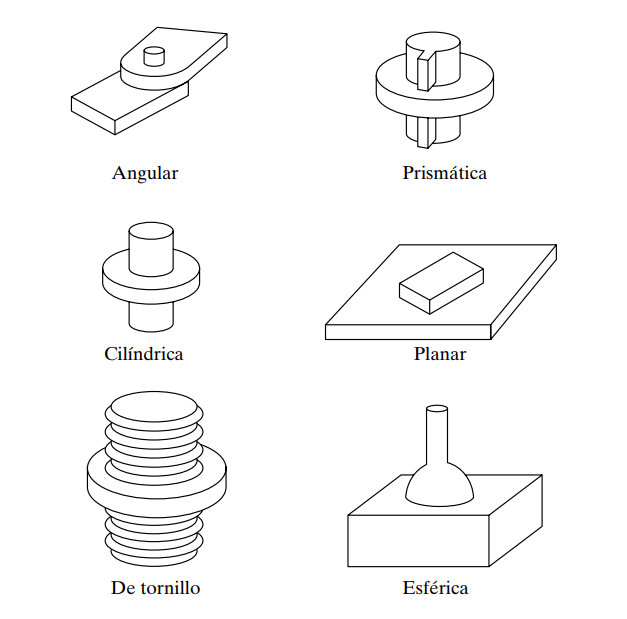
\includegraphics[width=0.5\textwidth, height=0.375\textheight]{./figs/6Articulaciones}
\caption{Tipos de mecanismos}
\label{mecanismos}
\end{figure}

Los movimientos que pueden realizar cada articulación de manera independiente se le denomina grado de libertad (GDL).
\begin{itemize}
\item La articulación angular permite que dos eslabones giren, uno respecto del otro, alrededor del eje de articulación; tiene 1 GDL.
\item La articulación prismática permite que dos eslabones arreglados en pares se deslicen, uno respecto al otro a lo largo de su eje; tiene 1 GDL.
\item La articulación cilíndrica permite la rotación alrededor del eje de la articulación y el traslado independiente a lo largo de ella; tiene 2 GDL.
\item La articulación plana permite dos traslados a lo largo de dos ejes independientes del plano de contacto y una rotación alrededor del eje perpendicular del plano.
\item La articulación de tornillo permite que dos eslabones unidos giren alrededor del eje de la articulación y se trasladen, al mismo tiempo, a lo largo de él; consta de 1 GDL.
\item La articulación esférica permite que uno de los eslabones pareados gire libremente en todas las orientaciones posibles respecto al otro alrededor del centro de una esfera; tiene 3 GDL.\\
\end{itemize}

\textbf{Grado de libertad}\\
Formalmente un grado de libertad de un sistema mecánico se define como el número de coordenadas mínimas necesarias para describir perfectamente su posición o configuración. Así, un cuerpo rígido que se mueve en el espacio cartesiano tridimensional tiene seis GDL, tres para posición y tres para orientación.\\ 

\textbf{Cinemática de los robots}\\
La cinemática es un derivado de la física que estudia el movimiento sin considerar las fuerzas o pares que lo causan, es decir, estudia las leyes de movimiento sin tener en cuenta aspectos como masas e inercias. Estudia la trayectoria que tiene el robot a lo largo del tiempo, considerando la posición, velocidad y en ocasiones la aceleración. En otras palabras se puede decir que describe de manera analítica el movimiento espacial del robot como una función del tiempo.\\

\textbf{Cinemática Directa}\\
Se le conoce como a los modelos matemáticos que permiten calcular la posición de los eslabones de un robot a partir de sus componentes fijos y configuraciones de las articulaciones.\\
Se refiere al uso de ecuaciones para el cálculo de la posición del actuador final en un robot articulado a partir de los ángulos y/o desplazamientos de las articulaciones o de la posición y orientación de las bases de un robot móvil a partir de las velocidades de las ruedas.\\

\begin{figure}[!h]
\centering
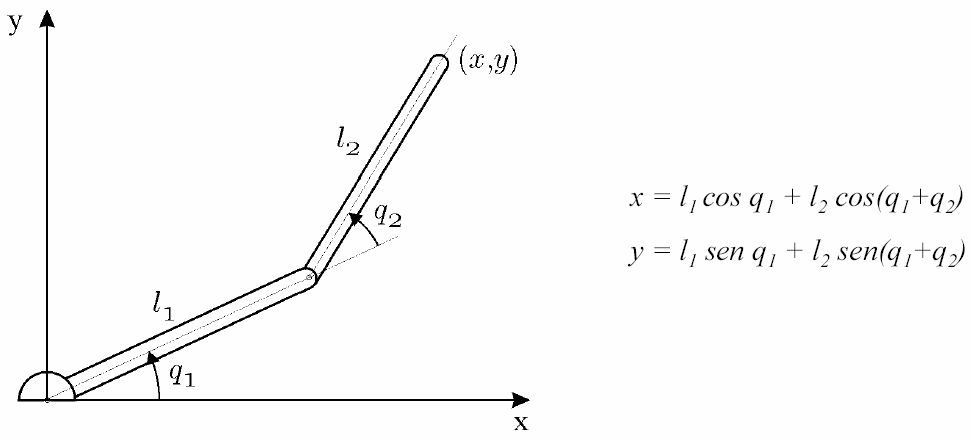
\includegraphics[width=0.7\textwidth, height=0.25\textheight]{./figs/robot2GDL_cinematica_directa}
\caption{Robot de 2GDL}
\label{robot2gdl}
\end{figure}

\newpage
\textbf{Cinemática Inversa}\\
Es el proceso inverso por el cual se obtienen modelos matemáticos que permiten, a partir de una posición y/o desplazamientos de los actuadores. Por lo general podemos encontrar configuraciones que no son factibles, es decir, que no son alcanzables, soluciones múltiples, ya sea que el robot ejerza un movimiento con codo hacia arriba o con codo hacia abajo.

\begin{figure}[!h]
\centering
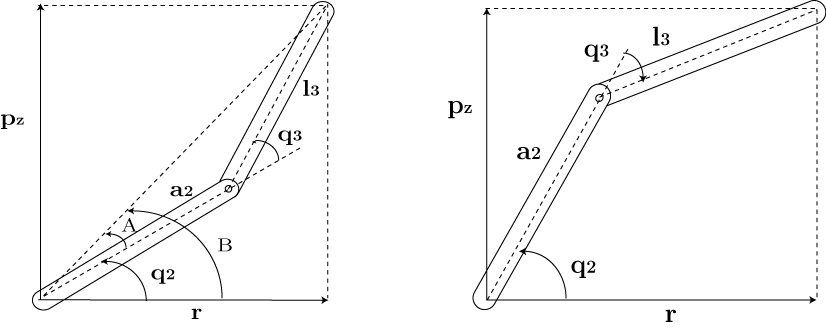
\includegraphics[width=0.8\textwidth, height=0.27\textheight]{./figs/codoarribaabajo}
\caption{Codo hacia abajo y hacia arriba}
\label{codos}
\end{figure}

Los problemas de la cinemática inversa suelen usar métodos aproximados para el cálculo de las variables de articulación, por ejemplo, a partir de la pseudo-inversa de la matriz Jacobiano. Para el caso de un robot articulado con 6GDL, la solución exacta pasa por desacoplar los tres primeros ejes de los tres últimos. En este sentido, la posición del efector final determina los valores de los tres primeros ejes, mientras que la orientación del efector final determina los valores de las tres últimas articulaciones.\\

\textbf{Metodología de Denavit-Hartenberg}\\
La metodología de Denavit-Hartenberg (D-H) permite establecer la ubicación de los sistemas de referencia de los eslabones en los sistemas robóticos articulados, ya sean prismáticas o de revolución, con cadenas cinemáticas abiertas. Jacques Denavit y Richard Hartenberg introdujeron esta convención en 1955 con el propósito de estandarizar la ubicación de los sistemas de referencia de los eslabones de un robot.\\

\newpage
\textbf{Parámetros D-H}\\
Se trata de una metodología ampliamente utilizada en el ámbito académico y de investigación en robótica que permite definir las transformaciones relativas entre eslabones con tan solo cuatro parámetros siento éste el número mínimo de parámetros para configuraciones genéricas.\\


La metodología de D-H define cuatro transformaciones que se aplican de forma consecutiva.
\begin{itemize}
\item d: Desplazamiento a lo largo de z anterior a la normal común.
\item $\theta$: Ángulo sobre la z anterior, de la x anterior a la nueva x.
\item l: Longitud de la normal común. Suponiendo una articulación revoluta, este es el radio de z anterior.
\item $\alpha$: Ángulo sobre la normal común, del antiguo eje z al nuevo eje z.
\end{itemize}

El contenido anterior fue obtenido del libro de \textit{Introducción a la robótica} \cite{saha-2010} de Subir Kumar Saha y de \textit{Fundamentos de la robótica} \cite{barrientos-2007} de A. Barrientos, L. Peñin, C. Balaguer, R. Aracil.\\

\textbf{SolidWorks}\\
SolidWorks es un programa de diseño que consiste en la especificación de puntos, líneas, curvas o superficies a través de un conjunto de parámetros iniciales y de las relaciones existentes entre ellos. Para el diseño, el modelado paramétrico es un recurso muy importante ya que proporciona ventajas como reducir el tiempo y esfuerzo que se requieren al modificar y realizar variaciones en éste y elimina tareas repetitivas al realizar variantes en el diseño.\\

En el programa se crean tres tipos de archivos: piezas, ensambles y dibujo. Además estos archivos están relacionados entre sí, es decir, cuando se realiza la modificación del dibujo, ésta afecta automáticamente a todos los archivos donde se encuentra referenciada la pieza realizada. \cite{herrera-2016} \\

\newpage
\textbf{MatLab}\\
MATLAB es una de las muchas sofisticadas herramientas de computación disponibles en el comercio para resolver problemas de matemáticas, tales como Maple, Mathematica y MathCad. Cada una permitirá efectuar cálculos matemáticos básicos, pero difieren en el modo como manejan los cálculos simbólicos y procesos matemáticos más complicados, como la manipulación de matrices. Por ejemplo, MATLAB es superior en los cálculos que involucran matrices, mientras que Maple lo supera en los cálculos simbólicos. El nombre mismo de MATLAB es una abreviatura de Matrix Laboratory, laboratorio matricial. En un nivel fundamental, se puede pensar que estos programas son sofisticadas calculadoras con base en una computadora. Son capaces de realizar las mismas funciones que una calculadora científica, y muchas más.\\
En muchas clases de ingeniería, la realización de cálculos con un programa de computación matemático como MATLAB sustituye la programación de computadoras más tradicional. MATLAB se han convertido en una herramienta estándar para ingenieros y científicos. \cite{moore-2007}\\

\textbf{Simulink}\\
Simulink® 3D Animation ™ proporciona aplicaciones para vincular modelos Simulink y algoritmos MATLAB® a objetos gráficos 3D. Los objetos se pueden representar en los lenguajes de modelado 3D estándar X3D y VRML97. Puede animar un mundo tridimensional cambiando la posición, la rotación, la escala y otras propiedades del objeto durante el escritorio o la simulación en tiempo real. También puede detectar colisiones y otros eventos en el mundo virtual y alimentarlos de nuevo en sus algoritmos de MATLAB y Simulink. El video de las cámaras virtuales se puede transmitir a Simulink para su procesamiento.

Simulink 3D Animation incluye editores y visualizadores para renderizar e interactuar con escenas virtuales. Con 3D World Editor, puede importar formatos de archivos CAD y URDF, así como crear escenas detalladas ensambladas a partir de objetos 3D. El mundo 3D se puede ver de forma inmersiva con la visión estereoscópica. Puede incorporar múltiples vistas de escena en 3D dentro de las figuras de MATLAB e interactuar con el mundo virtual usando un joystick de retroalimentación forzada, un mouse espacial u otro dispositivo de hardware. \cite{mathw-2018} \\

\textbf{Java 3D}\\
Java 3D es una interfaz de programación de aplicaciones (API) desarrollada en Sun Microsystems para renderizar gráficos 3D interactivos utilizando el lenguaje de programación Java. Java 3D es una API de Java del lado del cliente. Otros ejemplos de API del lado del cliente de Sun incluyen Abstract Windows Toolkit (AWT) y Java Foundation Classes (JFC / Swing), que son ambas bibliotecas de clases Java para crear aplicaciones con una Interfaz gráfica de usuario (GUI). Las API de Java del lado del cliente contrastan con las API del lado del servidor de Sun tales como Enterprise Java-Beans (EJB) y los otros componentes de Java 2 Enterprise Edition (J2EE). 

La principal ventaja de los desarrolladores de Java 3D para Java es que les permite programar en Java al 100 por ciento. En cualquier aplicación 3D grande, el código de representación solo constituirá una fracción de la aplicación total. Por lo tanto, es muy atractivo tener código de aplicación, persistencia y código de interfaz de usuario (UI) en un lenguaje fácilmente portátil, como Java. \cite{selman-2002}\\

Megan Flanders \cite{flanders-2015} menciona que la realidad virtual está jugando un papel muy importante como herramienta educacional que hace mas tangible los conceptos para los estudiantes; concuerdo totalmente ya que una vez vistos los conceptos es mas sencillo aplicarlos en un programa y observar como se comportan de manera visual, además que se aprende a utilizar un software, se fortalece la teoría aplicándola de manera práctica en un programa.\\
En su artículo se observa que el menú es amigable con el usuario, fácil de interpretar y modificar las opciones para poder visualizar los resultados finales ya dentro del mismo simulador. Es la idea tomar en cuenta que como va orientado para alumnos, ellos tienen que comprender de la mejor manera los resultados arrojados por el mismo programa para que capten la teoría utilizando el software.\\
Se muestran resultados por parte de los alumnos ya que se realizaron encuestas los cuales mayormente el 55\% dicen que la herramienta sería una gran parte complementaria al curso, además el 61\% comenta que es fácil de usar el 61\% menciona que es mas fácil entender de manera interactiva con modelos en 3D que con dibujos en 2D, además se muestra que el 74\% comenta que ha incrementado ligeramente su conocimiento en estos temas.\\
Build-a-robot fue creado con MatLab y sus herramientas de VRLM para poder tener los modelos 3D. MatLab contiene muchas herramientas que facilitan a los ingenieros el poder simular, crear y desarrollar ideas, ya que cuenta con herramientas dentro del mismo programa que son complementarias y como corren dentro del mismo es mas sencillo tener acceso y combinarlas para poder crear un buen proyecto.\\

En el artículo de P. Abreu \cite{abreu-2015} habla sobre un laboratorio virtual a diferencia de lo que se quiere realizar este va enfocado a la industria, se tiene el mismo objetivo que es crear un simulador solo que este toma en cuenta además del robot maquinaria con la cual se desea trabajar, se simula el ambiente en el cual el robot estará operando y se puede llegar a una conclusión de si será optimo usar al robot para dicha etapa de producción o a lo que se requiera llevar a cabo. RobotStudio tiene un menú algo mas complicado en el aspecto que a comparación del de Megan y lo que se desea hacer este tiene un teach pendant y un distinto ambiente virtual, está lleno de símbolos, muestra la pantalla del teach pendan y los diferentes menús para poder utilizar el simulador, toman diferentes caminos, como se ha mencionado está hecho para un ambiente más robusto que enfoca otras características.
